\documentclass[12pt, paper=a4]{article}
\usepackage[utf8]{inputenc}
\usepackage[german]{babel}
\usepackage{amsmath}
\usepackage{amssymb}
\usepackage{listings}
\usepackage{enumitem}
\usepackage{graphicx}
\usepackage{fancyhdr}

\author{Benjamin Cordt, xxxxxxx\\Paul Hölzen, 6673477\\Ino xx, xxxxxxx}

\title{GWV Hausaufgaben 1}

\rhead{B. Cordt, P. Hölzen, I. xx}
\pagestyle{fancy}
\begin{document}
\maketitle

\section*{Aufgabe 1.1}
\begin{itemize}
\item Fully observable $\Leftrightarrow$ partially observable\\
      Eine AI Applikation muss unter Berücksichtigung der Beobachtbarkeit der Welt entworfen werden, da
      nicht beobachtbare Komponenten einen großen Einfluss auf die Umwelt und damit auf das Verhalten der
      AI haben können bzw. sollten.\\
      Ein Problem, das in einer nur teilweise beobachtbaren Welt besteht, nicht aber in einer vollständig
      beobachtbaren, ist das mögliche Übersehen oder falsche Behandeln von unsichtbaren Einflüssen.
\item Discrete $\Leftrightarrow$ continuous\\
      Wenn von einer diskreten Welt ausgegangen wird, obwohl eine kontinuierliche vorliegt, können die
      ``Zwischenwerte'' nicht abgebildet oder verarbeitet werden.\\
      Ein Problem einer kontinuierlichen Welt gegenüber einer diskreten ist die Kathegorisierung von
      Ereignissen oder Werten, da diese zwischen Erwartungs-/Schwellwerten liegen können.
\item Deterministic $\Leftrightarrow$ stochastic
      In einer deterministischen Welt hat jede Aktion geau ein festes Ergebnis. Eine AI die mit diesem
      Konzept entworfen wurde, stößt in einer stochastischen Welt auf Probleme, sobald dieses Ergebnis
      abweicht.\\
      Dies ist auch das Problem einer stochastischen Welt im Gegensatz zur deterministischen: Reaktionen
      auf die Umwelt und müssen sehr flexibel sein um auch unvorhergesehene Ergebnisse verarbeiten zu
      können.
\end{itemize}

\section*{Aufgabe 1.2}
\subsection*{1.}
\subsection*{2.}
a)\\
Gegeben ist ein Rätsel, man hat eine 4 Liter Krug und einen 3 Liter Krug die aber nicht beschriftet sind. Man kennt nur den maximalen füllstand. Das Ziel ist es so in den 4 Liter Krug 2 Liter Wasser unterzubringen. Die erlaubten Handlungen sind:\\
\begin{enumerate}
\item Einen Krug, an der Pumpe, komplett aufzufüllen. Egal wie voll er schon bis dahin ist.
\item Einen Krug auszukippen. Den Inhalt auf 0L bringen
\item Den Inhalt eines Kruges in den anderen zu kippen und zwar bis der andere voll ist oder der erste leer.
\end{enumerate}
Der Inhalt eines Kruges kann nur ganzzahlige Werte von 0 bis 4 bzw. 0 bis 3 annehmen.\\

\begin{align*}
&State: &<4l Krug, 3l Krug>\\
&goal: &<2,?>\\
&start: &<0,0>\\
\end{align*}

\begin{figure}[h!]
\centering
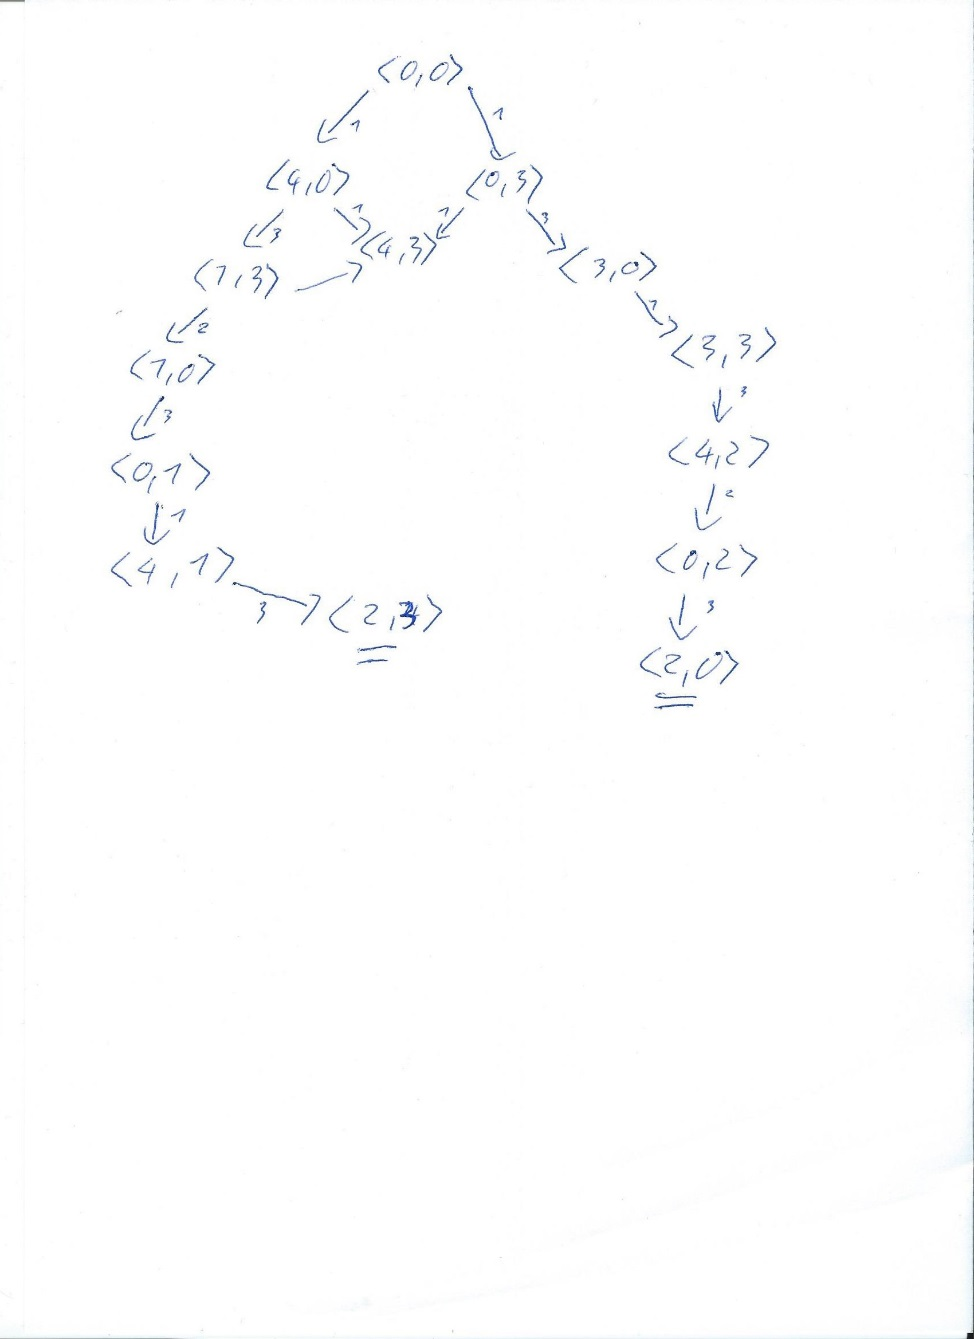
\includegraphics[scale=0.7]{tree.jpg}
\end{figure}
\newpage

In der Graphik sieht man die möglichen zustände und die Pfade die zum Ziel führt.\\

Die Zahlen an den Kanten stehen für die Möglichen Handlungen die man durchführen kann. Theoretisch kann man aus einem Zustand in den vorigen zurückkehren.\\

\noindent b)\\
Das selbe Rätsel wie in Teileaufgabe a, nur ist hier die 2 Handlung nicht mehr möglich. Man darf den Inhalt eines Kruges nicht wegkippen. Dies führt dazu, dass der Trick mit den hin und her schütten nicht mehr funktioniert, da der das wegschütten von Wein voraussetzen würde und da wir nur den Zustand des Kruges kennen wenn er voll, leer und danach folgende Zustände (hin und her schütten) aufgrund der ersteren Zustände kennen, gibt es keine Möglichkeit mehr auf genau zwei Liter zu kommen.

\end{document}
